\section*{Bakteriorhodopsin Konzentration}


Um die Bakteriorhodopsin Konzentration zu bestimmen, muss zunächst die Extinktion bestimmt werden. Dafür werden die Daten aus der Absoprtionsmessung analysiert.

\subsection*{Extinktion}
Zunächst muss jedoch die Streuintensität abgezogen werden, dafür wird eine Baseline Intensität bestimmt.


Die Basline wir mithilfe von Matlab geffited um eine genauere Approximation zu erhalten.
Die Form der Baseline ist 
\begin{equation*}
    I_{\mathrm{Background}} = a \cdot x^4 + b
\end{equation*}

Angehangen sind die Ergebnisse des Fits, zur Datenermittlung wurde ein Edgefinder auf das Bild des Spektrums angewandt.
Die Daten wurden dann händisch aussortiert und nur die Schawarzen Datenpunkte zum fitten verwendet.

\begin{figure}[htbp]
    \centering
    
    \begin{subfigure}[b]{0.3\textwidth}
        \centering
        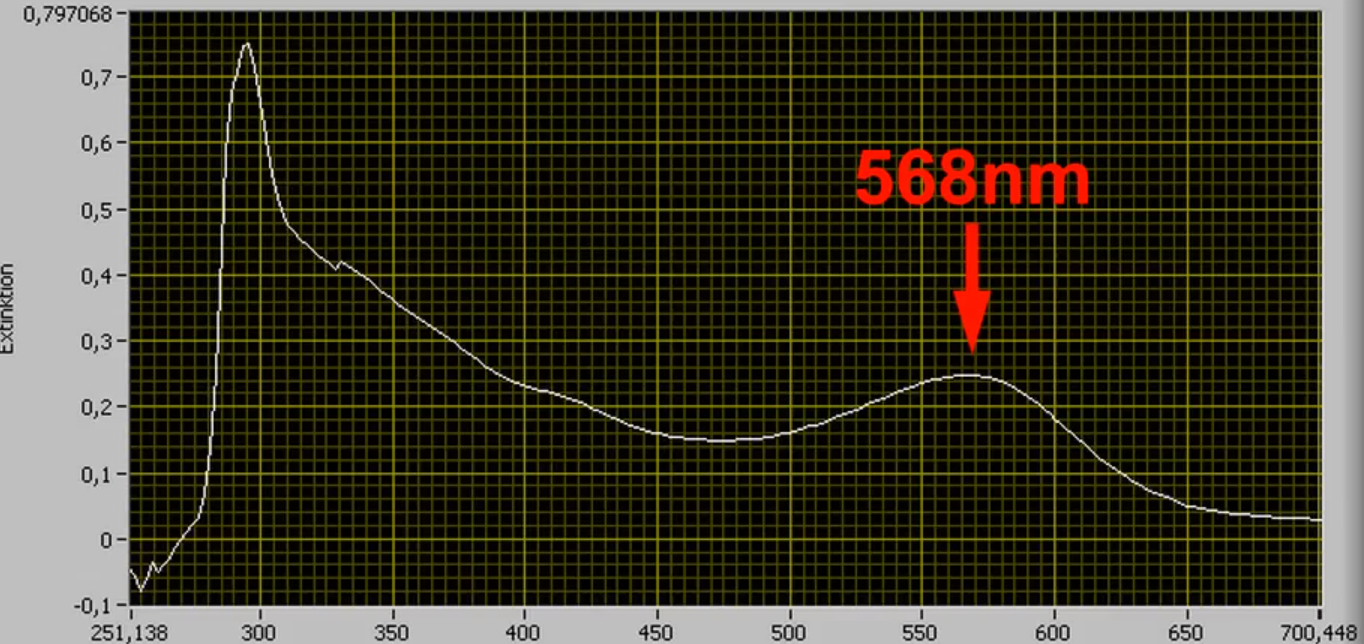
\includegraphics[width=\textwidth]{Spektrum.png}
        \caption{Spektrum der Absoprtionsmessung}
        \label{fig:Spektrum}
    \end{subfigure}
    \hfill
    \begin{subfigure}[b]{0.3\textwidth}
        \centering
        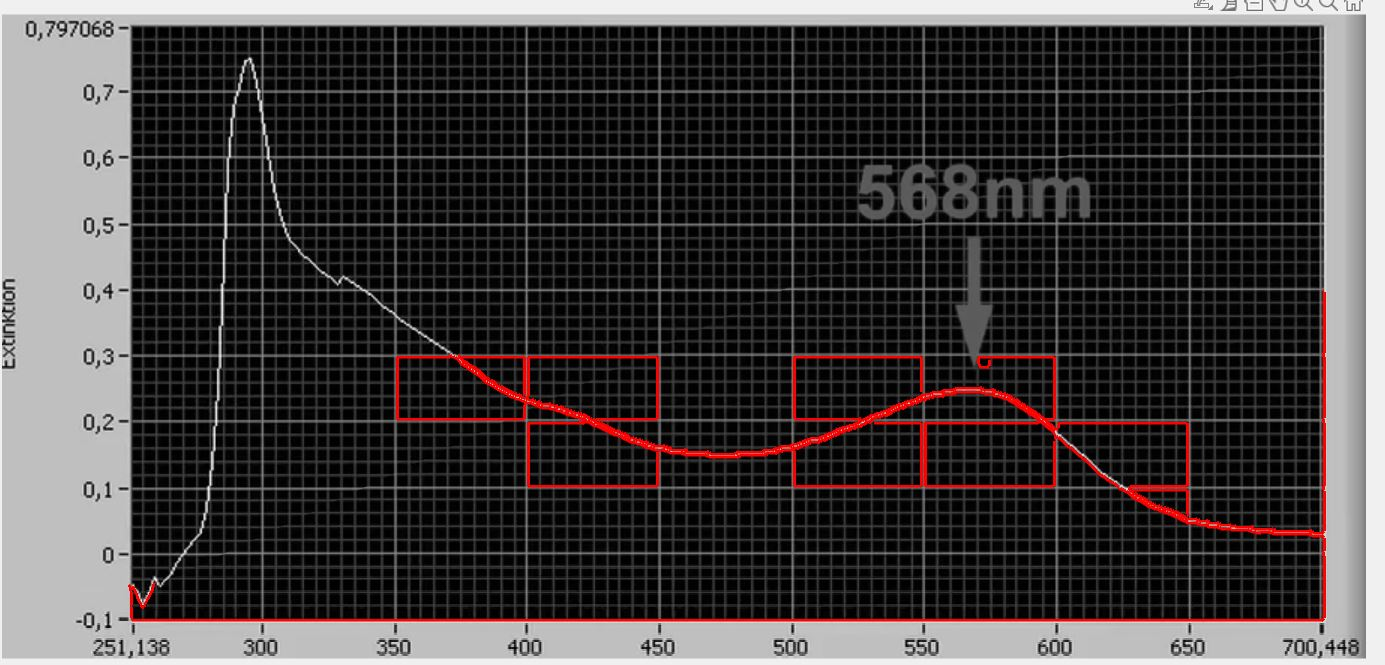
\includegraphics[width=\textwidth]{Data picture.JPG}
        \caption{Detektion der Daten}
        \label{fig:Datafind}
    \end{subfigure}
    \hfill
    \begin{subfigure}[b]{0.3\textwidth}
        \centering
        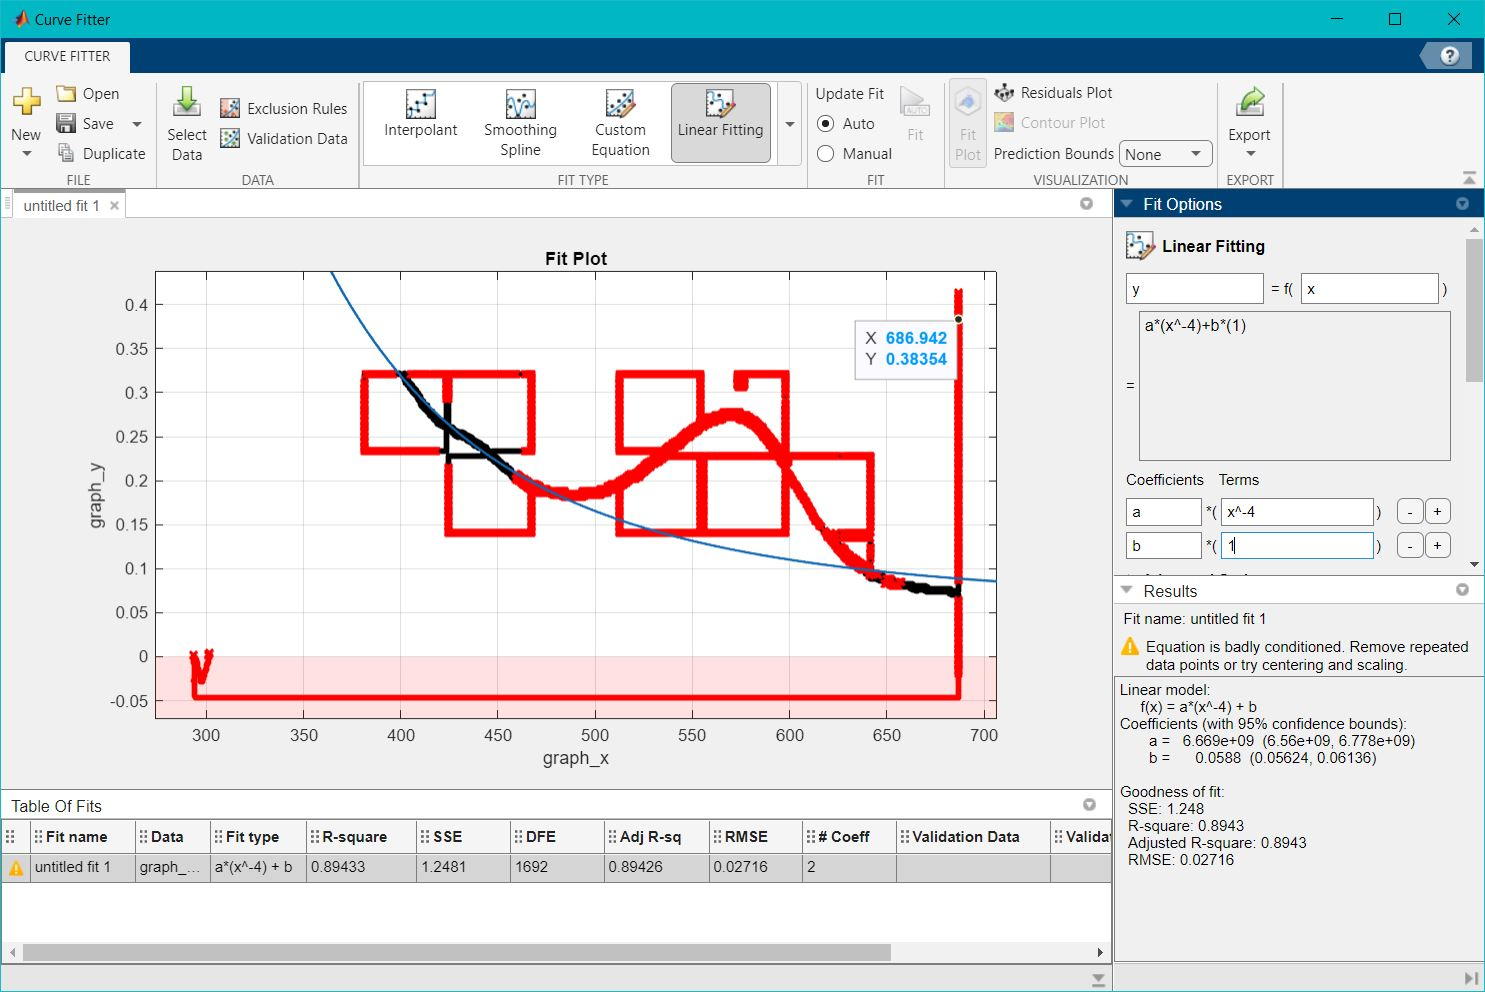
\includegraphics[width=\textwidth]{matlab fit.JPG}
        \caption{Fit des Hintergrunds}
        \label{fig:Fit}
    \end{subfigure}
    
    \caption{Prozess um Hintergrund zu bestimmen}
    \label{fig:Background}
\end{figure}

Der daraus ermittelte Wert für den Hintergrund ist
\begin{align*}
    y_{\mathrm{Background}} = 0,1229.
\end{align*}

Der Wert für die Extinktion ergibt sich aus der Differenz der Daten 
\begin{equation}
    E_{\mathrm{Peak}} = 0,2773 - 0,1229 = 0,1544
\end{equation}


\subsection*{Konzentration der bR Probe}


Zur bestimmung wird das Lambert-Beerschen Gesetz verwendet und umgestellt
\begin{align*}
    E &= \epsilon \cdot c \cdot d,\\
    c &= \frac{E}{\epsilon \cdot d}
\end{align*}


 mit
\begin{align*}
   \epsilon = \SI{63.000}{\L\per\mole\per\cm}, \; \text{und} \; d = \SI{1}{\cm}.
 \end{align*}


 Die Konzentration in der die Messung vorgenommen wurde ist daher
 \begin{equation*}
    c = \SI{2,45e-6 }{\mole\per\L}
 \end{equation*}

 Da der Überstand vorher mit Wasser im Verhältniss 1:5 verdünnt wurde beträgt die eigentliche
 Konzentration des Überstandes das fünffache also
 \begin{equation*}
    c_{\mathrm{Ueberstand}} = \SI{1,225e-5}{\mole\per\L}
 \end{equation*}

Die Konzentration des Überstandes ist nochmal verschieden von der Konzentration in der Bakterienpaste.
Um den Überstand zu erhalten wurden $\SI{200}{\micro\L}$ Paste mit $\SI{1}{\ml}$ Wasser und $\SI{200}{\micro\L}$ DNAse verdünnt.
Das Wasser dient hierbei als Auslöser eines osmotischen Schock wodurch die Zellen aufplatzen.
Die DNAse wird hierbei hinzugefügt um die Restliche DNA der Zellen aufzulösen und die Viskosität der Probe zu verringern.
Dadruch ist es auch einfach die Lösung vorsichtig zu durchmischen.
Dies ergibt ein Verhältnissvon 1:7. Daher ist die Konzentration der Paste 
\begin{equation*}
    c_{\mathrm{Paste}} = \SI{8,575e-5}{\mole\per\L}
\end{equation*}
Die Menge an Bakteriorhodopsin in dem Überstand kann durch einfach bestimmt werden mithilfe der Konzentration und des Volumens
\begin{equation*}
    n = \SI{200}{\micro\L} \cdot \SI{8,575e-5}{\mole\per\L} = \SI{1,7715e-8}{\mole}.
\end{equation*}

Analog dazu lässt sich die Masse des Bakteriorhodopsin bestimmen
\begin{equation*}
    m = \SI{1,7715e-8}{\mole} \cdot \SI{26e3}{\g\per\mole} = \SI{0,461}{\milli\g}
\end{equation*}
